\documentclass{article}

\usepackage{graphicx}
\usepackage[utf8]{inputenc}
\usepackage[english]{babel}
\usepackage[document]{ragged2e}



\begin{document}

\textbf{Q1}  
\textbf{) Image Sharpening}
\vskip 0.2in

Pranav Sankhe \texttt{150070009} \newline
Kalpesh Krishna \texttt{140070017}  \newline
Mohit Madan \texttt{15D070028} \newline

\vskip 0.5in

\textbf{Report:}  
\vskip 0.1in

Here are the results for image \texttt{lionCrop.mat}:

\begin{figure}[h!]
  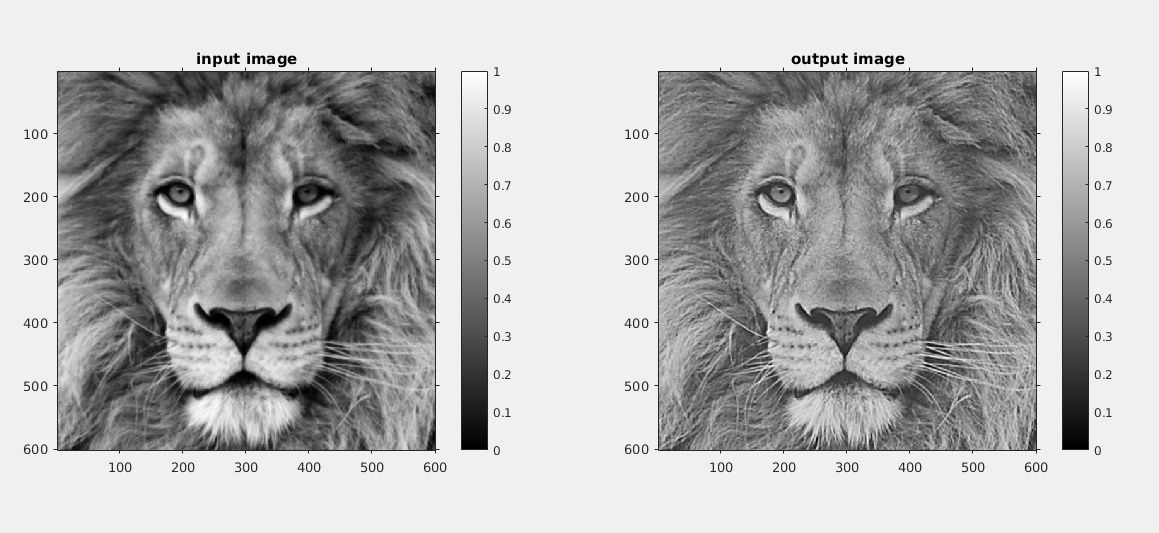
\includegraphics[width=\linewidth]{lion_result.png}
  \caption{Original and Sharpened images}
  \label{fig:result1}
\end{figure}

Here are the results for image \texttt{superMoonCrop.mat}:

\begin{figure}[h!]
  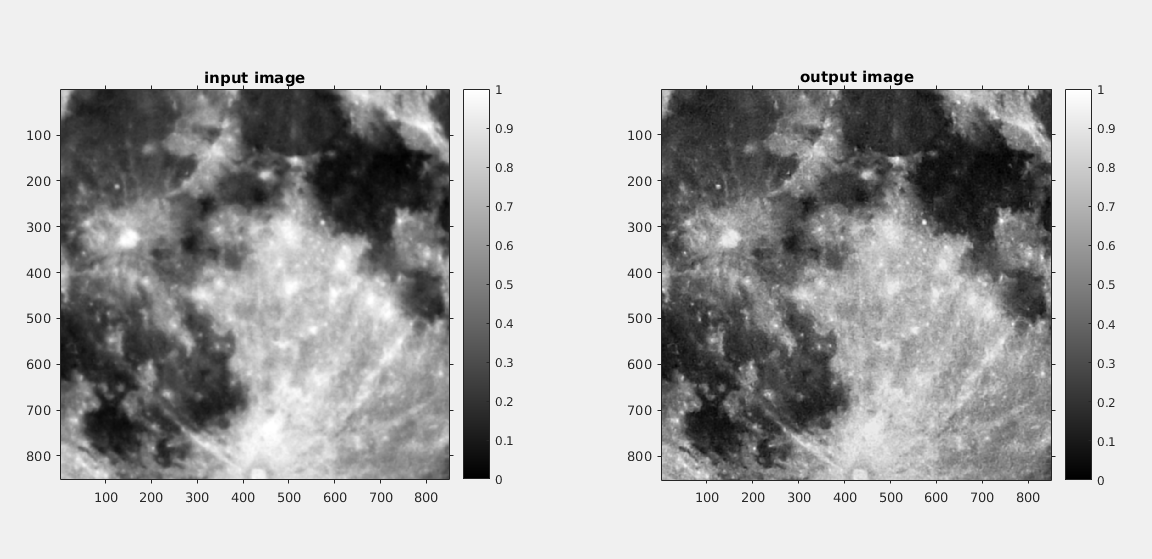
\includegraphics[width=\linewidth]{moon_result.png}
  \caption{Original and Sharpened images}
  \label{fig:result2}
\end{figure}

\newpage
\textbf{Optimal parameters} values are as follows: \newline
For image =  \texttt{lionCrop.mat} : \newline
\texttt{standard deviation = 2 }  \newline
\texttt{scaling factor = 2.5 }

\vskip 0.2in

For image =  \texttt{superMoonCrop.mat} : \newline
\texttt{standard deviation = 2 } \newline
\texttt{scaling factor = 3 }

\vskip 0.2in


\end{document}